% \documentclass[conference]{IEEEtran}
\documentclass[conference,compsoc]{IEEEtran}
% \documentclass[journal]{IEEEtran}
% \documentclass[10pt,journal,compsoc]{IEEEtran}
% \documentclass[journal,comsoc]{IEEEtran}
% \documentclass[journal,transmag]{IEEEtran}

\usepackage[utf8]{inputenc}
\usepackage[T1]{fontenc}
\usepackage[ngerman]{babel}
\usepackage{ifpdf}

\ifCLASSOPTIONcompsoc
  % \usepackage[nocompress]{cite}
  \usepackage[numbers,sort]{natbib}
\else
  \usepackage{cite}
\fi

\ifCLASSINFOpdf
  \usepackage[pdftex]{graphicx}
  \graphicspath{{../pdf/}{../jpeg/}}
  \DeclareGraphicsExtensions{.pdf,.jpeg,.png}
\else
  \usepackage[dvips]{graphicx}
  \graphicspath{{../eps/}}
  \DeclareGraphicsExtensions{.eps}
\fi

\usepackage{amsmath}
\usepackage{algorithmic}
\usepackage{array}

\ifCLASSOPTIONcompsoc
  \usepackage[caption=false,font=footnotesize,labelfont=sf,textfont=sf]{subfig}
\else
  \usepackage[caption=false,font=footnotesize]{subfig}
\fi

\usepackage{stfloats}
\usepackage{float}
\usepackage{url}

\hyphenation{op-tical net-works semi-conduc-tor}

\begin{document}
\title{Heiligt der Zweck die Mittel? - Wie werden Entscheidungen beim autonomen Fahren getroffen}

\author{
  \IEEEauthorblockN{Christoph Stach}
  \IEEEauthorblockA{
    Hochschule für Technik und Wirtschaft Berlin\\
    Fachbereich 4 - Angewandte Informatik\\
    s0555912@htw-berlin.de
  }
}

\maketitle

\begin{abstract}
    Autonomes Fahren ist ein noch relativ junges Forschungsfeld. Neue technologische Fortschritte machen es möglich, dass sich Fahrzeuge gänzlich ohne oder nur mit minimaler menschlicher Überwachung eigenständig auf Straßen oder in dafür vorgesehen Umgebungen bewegen können. Doch welche Gefahren bestehen beim autonomen Fahren und wer entscheidet in auftretenden Ernstfällen über den Ausgang einer Extremsituation? Das sind u. a. Fragen mit denen sich derzeit Wissenschaft und Gesellschaft gleichermaßen intensiv beschäftigten. Mit dieser Arbeit möchte der Author einen kurzen allgemeinen Überblick über das Themengebiet geben, z. B. welche Technologien zum Einsatz kommen, und versuchen, speziell das Treffen moralischer Entscheidungen in Extremsituation beim autonomen Fahren in der EU getroffen werden.
\end{abstract}
\section{Einleitung}

Heutzutage wird der Großteil der Fahrzeuge auf unseren Straßen durch Menschen gesteuert. Doch das könnte sich bald ändern. Schon jetzt unterstützen Fahrassistenzsysteme die Fahrer und warnen unter Umständen in Gefahrensituationen.

Das Forschungsfeld des autonomen Fahrens besteht aus unterschiedliche Teilgebiete. In diesem Artikel wird  zwischen dem rein technischen Bereich und dem sozial-technischen Bereich unterschieden. Technologischen Forschungen beziehen sich auf Hardware, z.B. unterschiedliche Sensoren, und Software, z.B. Algorithmen und Assistenzsysteme, die benötigt werden um ein autonom fahrendes Fahrzeug zu realisieren. Der sozial-technische Bereich umfasst die Auswirkungen auf die Gesellschaft und das Vertrauen in die neuartige Technologie. Die Aspekte die durch autonomes Fahren entstehen werden versucht durch Gesetzgeber mit Richtlinien zu regulieren und Verfahren zu standardisieren. Dadurch entsteht zur Zeit ein internationaler Wettlauf um die Vorherrschaft in diesem Gebiet.

In dieser Arbeit gehen ich zuerst in \ref{sec:verwandte-literatur} auf  verwandte Arbeiten mit dem Thema ein. Ich stelle die unterschiedlichen wissenschaftlichen Arbeiten, die sich mit der Internetseite \textit{The Moral Machine}\footnote{\url{http://moralmachine.mit.edu/}} beschäftigen, vor. Danach beschäftige ich mich mit den wesentlichen Definitionen und Technologien in \ref{sec:definitionen-und-technologie}, die in autonomen Fahrzeugen zum Einsatz kommen, ein. Schließlich rege ich eine ethische Diskussion in \ref{sec:diskussion} an und begründe meine persönlichen Gedankengänge in einem Fazit in \ref{sec:fazit}.
\section{Verwandte Literatur}
\label{sec:verwandte-literatur}

Die Arbeit bezieht sich auf die Fachschriften der Internetseite \textit{Moral Machine Website}. Des weiteren wird unterschiedliche Grundlagenliteratur, die sich mit allgemeinen Begriffen und Technologien des autonomen Fahrens beschäftigt, vorgestellt.\\

\citeauthor{roadblocks} identifizieren in ihrer wissenschaftlichen Publikation \textbf{Psychological roadblocks to the adoption of self-driving vehicles \cite{roadblocks}} unterschiedliche Dilemmas und auftretende Herausforderungen, deren sich die Gesellschaft stellen muss. Entscheidungsträger werden Richtlinien für diese Dilemmas finden müssen die gleichermaßen von der Gesellschaft akzeptiert werden müssen. Hierfür werden mögliche Lösungsvorschläge unterbreitet. 

Es wird identifiziert, dass die Mehrheit ein Verhalten von autonomen Fahrzeugen in Extremsituationen das dem Gesamtwohl zu gute kommt bevorzugen würde. Kaufen würden Personen jedoch Fahrzeuge die Ihnen selbst möglichst hohe Sicherheit gewährleisten. Diese beiden Fakten schließen sich gegenseitig aus.

Unausweichliche Unfälle autonomer Fahrzeuge werden zu Überreaktionen in der Gesellschaft führen, was die Einführung und Annahme verlangsamen oder lahm legen könnte.

Durch die Verwendung von Anwendungen aus dem Bereich des Maschinellen Lernens kann den Entscheidungsprozess, den autonome Fahrzeuge in bestimmten Situationen treffen, schlecht nachvollzogen werden. Das kann dazu führen, dass ein allgemeines Misstrauen gegenüber der Technologie entsteht.\\

In \textbf{The Social Dilemma of Autonomous Vehicles \cite{socialDilemma}} beschreiben \citeauthor{socialDilemma} die Ergebnisse einer Studie mit 1929 Teilnehmern. Diese wurden dazu befragt ob sie Fahrzeuge mit einem zweckorientierten Verhalten in Extremsituationen bevorzugen und ob sie diese kaufen würden. Damit baut die Publikation auf dem bereits identifizierten ethischen Dilemma aus \cite{roadblocks} auf. Über Auswertungen wird gezeigt, dass eine Regulierung von autonomen Fahrzeugen durch den Gesetzgeber zu einem zweckorientierten Verhalten die Einführung verlangsamen würde. Das hätte in der Gesamtheit mehr Todesfälle zur Folge als die frühe Einführung der Technologie, da langfristig mehr Unfälle durch Menschen verursacht werden als durch autonome Fahrzeuge. 90\% der Unfälle sind auf menschliche Fehler zurückzuführen.\\

Der Artikel \textbf{The Moral Machine experiment \cite{moralMachine}} von \citeauthor{moralMachine} untersucht die Daten, die über die eine weltweit verfügbare Umfrageplattform \textit{The Moral Machine} gesammelt wurden. Nutzer wurden nach dem moralisch besser vertretbaren Ausgang verschiedener unausweichlicher Unfallszenarien befragt. Zur Auswahl hat ein Nutzer jeweils zwei unterschiedliche Ausgänge in eine Extremsituationen. Bei den Ausgängen müssen entweder die Insassen des Fahrzeugs, oder Passenten auf der Straße sterben. In den Szenarien werden auf der Straße und im Fahrzeug jeweils unterschiedliche Personengruppen abgebildet. Jedes Unfallszenarium stellt dabei ein ethisches Dilemma dar. Es wurden unterschiedliche Statistiken erhoben auf die in dieser Arbeit referenziert wird. Außerdem über Beobachtungen ein Unterschied in der moralischen Bewertung der Unfallszenarien in verschiedenen Kulturkreisen identifiziert. Es wird dabei wesentlich zwischen westlichem, südlichem und östlichem Kulturkreis unterschieden. Gesamtheitlich wurde beobachtet, dass es starke Präferenzen der Befragten zum \textit{Retten von Menschen (gegenüber Tieren)}, zum \textit{Retten von vielen Leben (gegenüber weniger Leben)} und zum \textit{Retten von jungen Menschen (gegenüber alten Menschen)} gibt. Zum Zeitpunkt der Erstellung des Artikels, \citeyear{moralMachine}, wurden 39,61 Millionen Entscheidungen aus 233 Ländern weltweit gesammelt. \\

\textbf{A Voting-Based System for Ethical Decision Making \cite{votingBasedSystem}}, verfasst von \citeauthor{votingBasedSystem}, schlägt einen Algorithmen, mit dem ethische Entscheidungen in Extremsituationen getroffen werden können, vor. Es handelt sich dabei auf einen technischen Algorithmus, der anhand der Daten die von \textit{The Moral Machine} gesammelt wurden, Entscheidungen treffen kann. Der Algorithmus wertet die Ergebnisse aller Teilnehmern der Plattform aus, führt diese zusammen und ist in der Lage  \textit{swap-dominance efficient} das finden von Alternativen zu erlernen. Methoden des Maschinellen Lernens werden verwendet und der trainierte Algorithmus ist in der Lage, die ethisch am besten zu akzeptierenden Ausgänge für eine Extremsituationen aus einer Menge von Alternativen zu finden.\\

Neben der Literatur von \textit{The Moral Machine} baut dieses Arbeit auf unterschiedlichen Grundlagewerken zum Thema des autonomen Fahrens auf. Der vom \citeauthor{smith2015automated} veröffentlichte Bericht \textbf{Automated and
autonomous driving: regulation under uncertainty \cite{smith2015automated}} beschreibt allgemeine Technologien und Terminologien der Domäne.\\

Außerdem werden die SAE-Level des Standard \textbf{Taxonomy and Definitions for Terms Related to Driving Automation Systems for On-Road Motor Vehicles \cite{standardSAE}} der \citeauthor{standardSAE} vorgestellt (siehe. \ref{ssec:sae-level}).\\
% \section{Akteure}
\label{sec:akteure}

Im Feld des autonomen Fahren tummeln such unterschiedliche Akteure. Einige nehmen passiv daran in dem Sie Richtlinie erstellen und Diskussionen anregen. Andere treiben aktiv die Weiterentwicklung in dem Bereich voran.

\subsubsection*{International Transport Forum} Das International Transport Forum (ITF)\footnote{\url{https://www.itf-oecd.org/}} ist ein unter dem OECD (Organisation for Economic Co-operation and Development) zwischenstaatliche Organisation die es sich zum Ziel gesetzt hat, ein tieferes Verständnis über das Transportwesen in Rollen des Wirtschaftswachstums, ökologischer Nachhaltigkeit und ethischen Aspekten zu fördern. Bestehend aus 60 Mitgliedsländern agiert es als Ideenschmiede für Richtlinie und organisiert das jährliche Gipfeltreffen der Transportminister. In unregelmäßigen Abständen veröffentlicht der ITF Berichte den verschiedenen Themen des Transportwesens.

\subsubsection*{Society of Automotive Engineers \cite{standardSAE}\cite{smith2015automated}} Das ITF stützt sich auf die von der Society of Automotive Engineers (SAE)\footnote{\url{https://www.sae.org/}}  definierten sechs Level des autonomen Fahrens. Diese reichen von komplett automatisierten Fahrzeugen bis hin zu komplett automatisierten Transportmittel, bei denen kein Fahrer mehr notwendig ist.\\


\section{Definitionen und Technologie}
\label{sec:definitionen-und-technologie}

In dieser Sektion werden die Grundlegenden Technologie und Definitionen beschrieben die zum Verständnis von autonomen Fahren wichtig sind.

\subsection{SAE-Level}
\label{ssec:sae-level}

Die SAE-Level \cite{standardSAE} beschreiben den Grad an Autonomie bei autonomen Fahrzeugen. Sie werden dabei in 6 unterschiedliche Stufen unterschieden und wurden von der \citeauthor{standardSAE} definiert.\\

\subsubsection*{Level 0 - Keine Automatisierung} Der Fahrer übernimmt die volle Kontrolle über das Fahrzeug.

\subsubsection*{Level 1 - Fahrassistenz} Der Fahrer wird durch einen einzelnen Fahrassistenten, z.B. Tempomat, Spurhalteassistent oder Bremsassistent, unterstützt, behält jedoch die volle Kontrolle über das Fahrzeug.

\subsubsection*{Level 2 - Partielle Automatisierung} Der Fahrer wird durch mehrere Fahrassistenten unterstützt and hat immer die Kontrolle über das Fahrzeug.
    
\subsubsection*{Level 3 - Bedingte Automatisierung} Das Fahrzeug ist in der Lage die Umgebung zu erkennen und ist in der Lage eigenständig in bestimmten Fahrsituationen zu meistern. Ein aufmerksamer Fahrer ist noch erforderlich, der unter Umständen einschreiten kann.

\subsubsection*{Level 4 - Hohe Automatisierung} Das Fahrzeug ist in der Lage sich eigenständig in den meisten Fahrumgebungen zu manövrieren. Es erkennt Fehlentscheidungen und kann auf diese reagieren. Menschliches einschreiten ist, wenn gewünscht, möglich.

\subsubsection*{Level 5 - Volle Automatisierung} Das Fahrzeug kann in allen Umgebungen und zu jederzeit und in jeder Situation komplett eigenständig Fahren.

\subsection{Sensoren}

In Autonomen Fahrzeugen kommen unterschiedliche Arten von Sensoren zum Einsatz. 
Dazu gehören Kameras, Radars, spezielle Laserscanner und Ultraschallsensoren.\\

\begin{figure}[H]
    \centering
    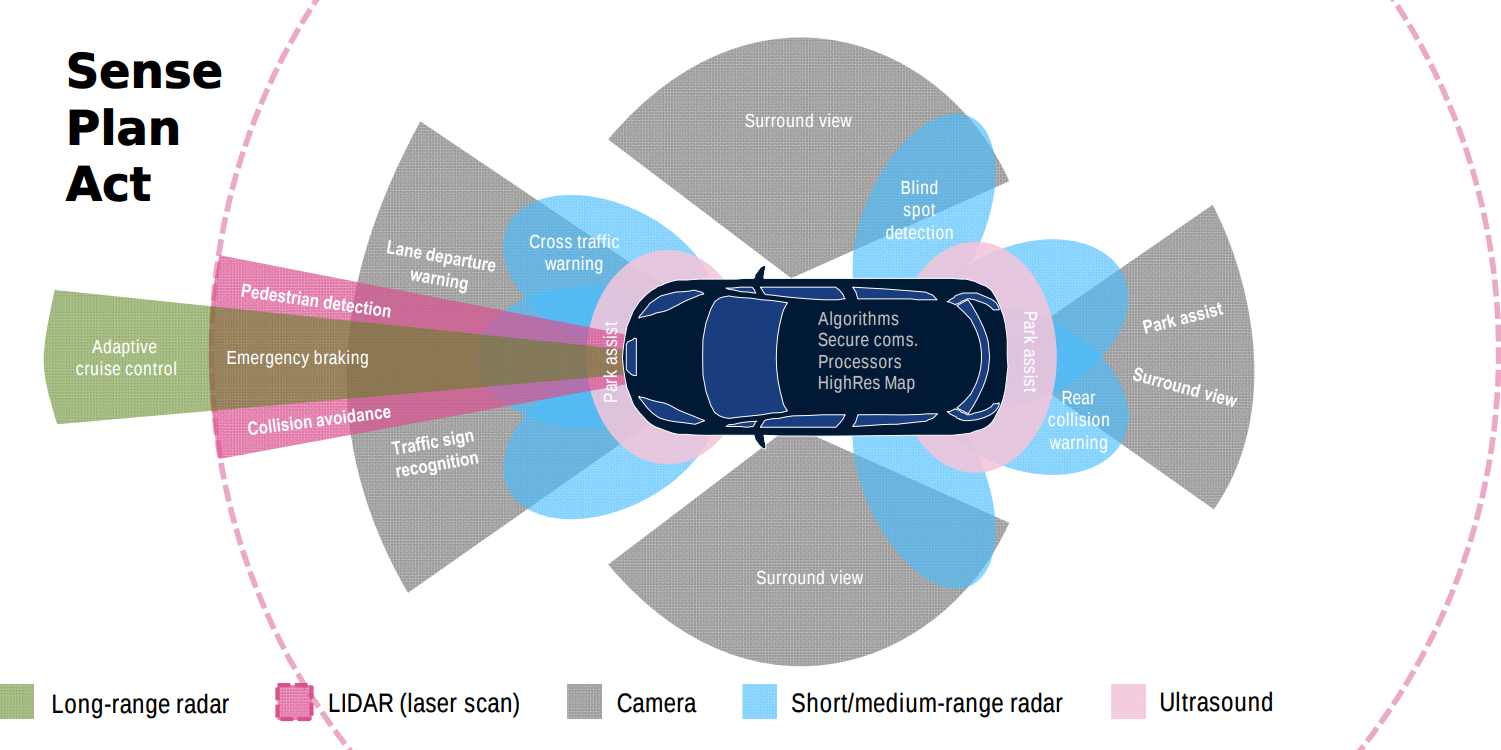
\includegraphics[width=.485\textwidth]{resources/images/sensors.png}
    \caption{Sensoren eines autonomen Fahrzeuges \cite{smith2015automated}}
\end{figure}

Kameras können rund um das Fahrzeug montiert werden und ermöglichen dem Fahrzeug somit eine vollumfängliche Sicht auf das Verkehrsgeschehen. Ein Vorteil gegenüber einem menschlichen Fahrer ist, das auch tote Winkel mit Kameras überwacht werden können. Lediglich durch die geschossenen Bilder der Kameras lässt sich jedoch die Entfernung zu erkannten Objekten schlecht einschätzen.\\

Hier kommt die LIDAR-Technologie \cite{himmelsbach2008lidar} ins Spiel. LIDAR steht für \textit{Light Detection and Ranging}. Es handelt sich um eine Umgebungsüberwachungstechnik die mit Hilfe eines Lasers Objekte in der Nähe bestrahlt und die Reflexion mit einem Sensor misst. So kann die Entfernung zu den Objekten berechnet werden.\\

Radar-Systeme \cite{introductionToRadarSystems} funktionieren ähnlich wie LIDAR-Systeme. Anstatt von Lichtwellen werden Radiowellen eingesetzt. Objekte in der Umgebung erzeugen ein Echo, welches vom einem Sensor empfangen wird. Somit ist ein Radar-System in der Lage die Distanz, Position und Geschwindigkeit von Objekten zu berechnen.\\

Ultraschall\\


\subsection{Vehicular Ad-hoc Network}

\begin{figure}[H]
    \centering
    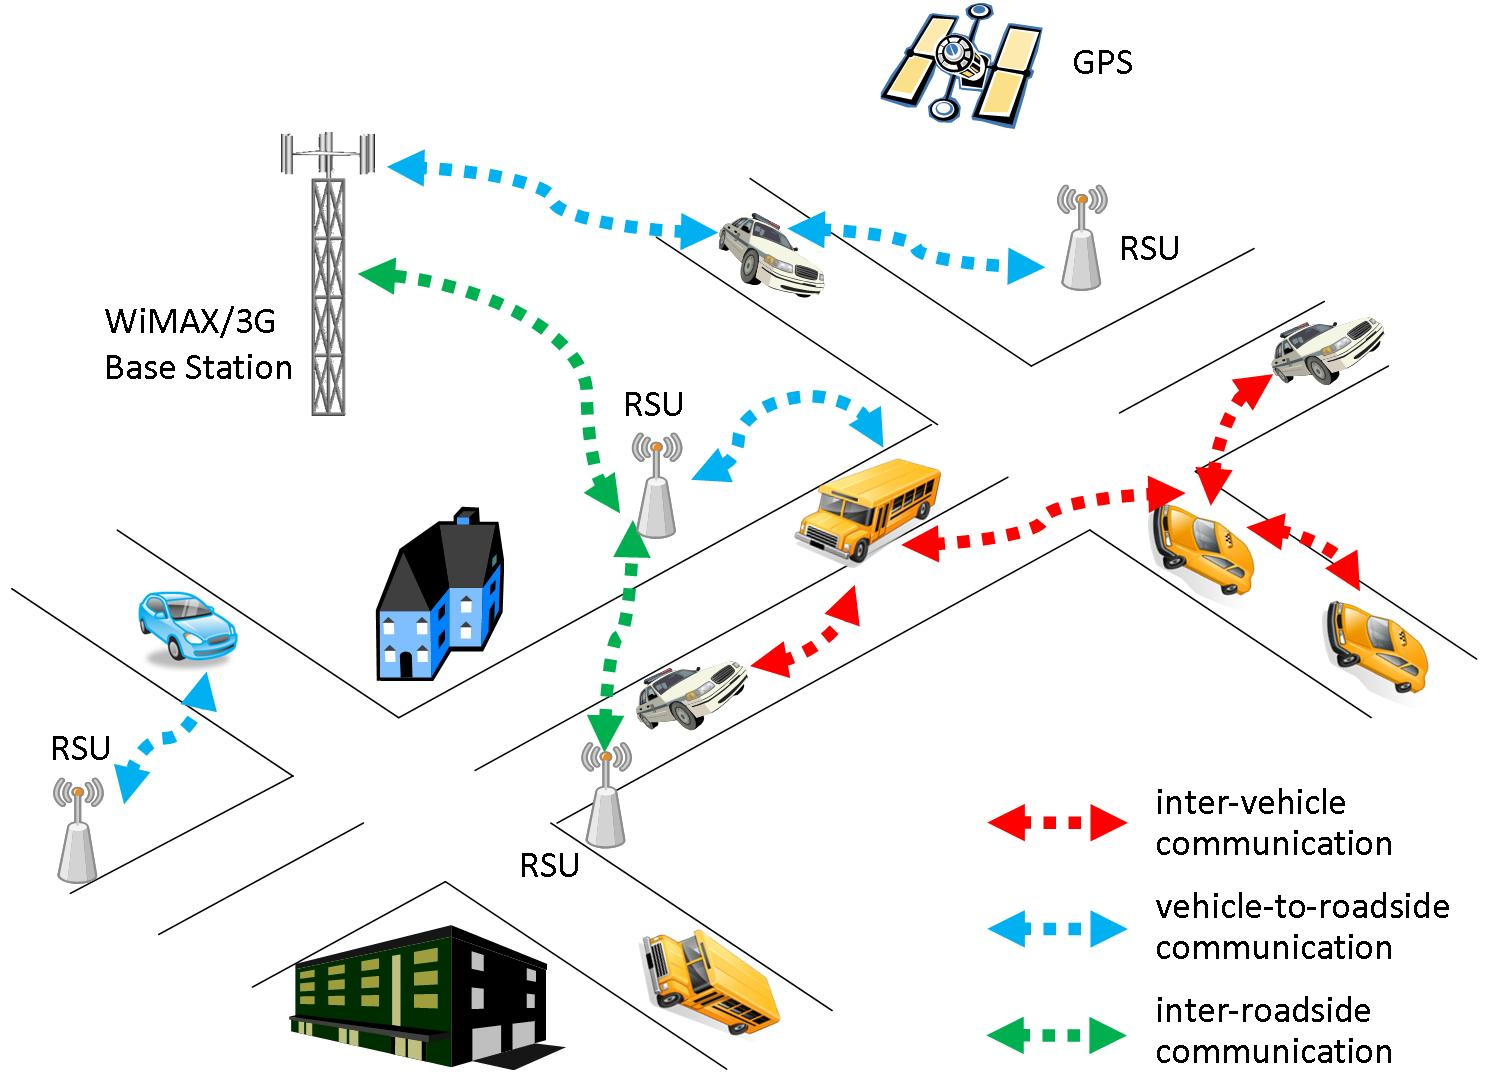
\includegraphics[width=.485\textwidth]{resources/images/vanet.jpg}
    \caption{Übersichtsgrafik eines VANETs \cite{vanet}}
\end{figure}

\subsection{Software}

\section{Diskussion}
\label{sec:diskussion}

Die Arbeit behandelt Fahrzeuge des SAE-Levels 4 und 5. Denn nur diese Fahrzeuge sind in der Lage ohne Supervision eines Fahrers sich im Straßenverkehr zu bewegen. 

\subsection{Vorteile}

Autonomes Fahren bringt viele Vorteile mit sich. Durch die unterschiedlichen Sensoren kann weitaus größeres Sichtfeld erzeugt werden, als es mit dem menschlichen Auge möglich ist. Software trifft Entscheidung binnen Millisekunden und kann akkurate Berechnungen über den Fahrtverlauf durchführen. 
Da es sich bei 90\% der Unfälle um menschliches Fehlverhalten handelt kann die durch die Einführung autonomer Fahrzeuge die Unfallrate dementsprechend gesenkt werden \cite{roadSafty}.

Durch die effiziente Kommunikation der Fahrzeuge untereinander können Staus vermieden werden. Der Verkehr würde sich besser auf unterschiedliche Teile des Verkehrsnetzes verteilen. Das verkürzt die Fahrzeiten insgesamt. 

Mit geteilten autonomen Fahrzeugen, die teil der öffentlich Verkehrsmittel werden, könnte die Anzahl der Fahrzeuge auf den Straßen insgesamt verringert werden. Die meiste Zeit stehen private Fahrzeuge auf Parkplätzen. Die Parkplatzsuche würde entfallen, was gerade in Großstädten ein bekanntes Problem ist. Eine Studie der Berryls Strategy Advisor zeigt das der Einsatz von 18.000 Robotertaxis den gesamten privaten Verkehr sowie 20\% des Pendlerverkehrs der Stadt München abdecken kann \cite{advisors2017simulation}.

Verkürzte Fahrtzeiten und weniger Fahrzeuge auf den Straßen wirkt sich auch positiv auf die Treibstoffemissionen aus. Somit würde der Einsatz von autonomen Fahrzeugen langfristig einen Beitrag zum Umweltschutz leisten.





\section{Fazit}
\label{sec:fazit}

\newpage

% \bibliographystyle{IEEEtranN-de}
% \bibliography{IEEEabrv,references/scientific,references/online,references/images}
\printbibliography

\end{document}